\section{Builder-Muster}

\paragraph{Problemstellung}
Sie haben soeben den Auftrag erhalten, einen Urlaubsplaner f"ur einen neuen Themenpark zur erstellen. Die G"aste des Parks k"onnen ein Hotel und verschiedene Sorten von Eintrittskarten ausw"ahlen, Tische in Restaurants servieren lassen und sogar Special Events buchen. Um den Urlaubsplaner zu erstellen, m"ussen Sie strukturen wie die folgenden erzeugen k"onnen. 

\begin{figure} [!htb]
	\centering
	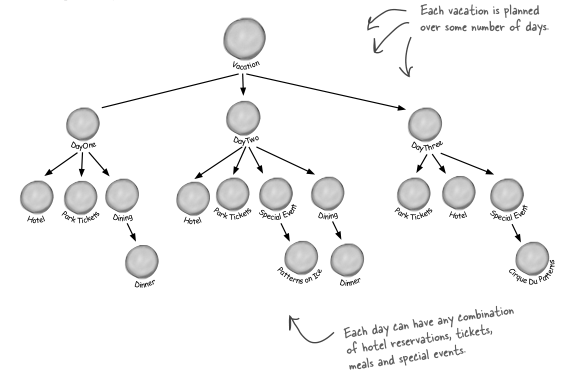
\includegraphics[width=.9\linewidth]{builder/img/builder}
	\caption{Darstellung der Datenstruktur}
	\label{fig:builder}
\end{figure}

Es soll besonders Wert auf eine flexible Datenstruktur gelegt werden, da verschiedene Besucher auch sehr verschiedene W"unsche haben. Zudem ben"otigen Sie eine Abfolge von m"oglicherweise komplexen Schritten f"ur die Erzeugung des Planers. Wie k"onnen Sie die komplexe Struktur erzeugen, ohne sie mit den Schritten f"ur die Erzeugung zu vermischen?

\paragraph{Erkl"arung des Musters}
\textbf{Definition:} Verwenden Sie das Builder-Muster, um die Konstruktion eines Produkts zu kapseln und seinen Aufbau in mehreren Schritten zu erm"oglichen.

"Ahnlichkeiten zum Iterator-Muster. Dort wurde die Iteration in einem separaten Objekt gekapselt und die interne Repr"asentation der Collection vor dem Client verborgen. Hier steckt der gleiche Gedanke dahinter: Wir kapseln die Erzeugung des Reiseplaners in einem Objekt (dem Builder oder Erbauer, hier nennen wir es Ersteller), und unser Client bittet dann den Ersteller, die Struktur des Reiseplaners f"ur ihn zu erstellen. Ein Blick in das folgende Diagramm sollte hierbei Klarheit verschaffen. 

\paragraph{Vorteile des Builder-Musters}
\begin{itemize}
	\item Kapselt die Art und Weise, wie ein komplexes Objekt hergestellt wird.
	\item Ermoglicht die Herstellung von Objekten in einem Prozess, der aus mehreren Schritten besteht und variiert (im Gegensatz zu Ein-Schritt-Fabriken).
	\item Verbirgt die interne Reprasentation des Produkts vor dem Client. 
	\item Produkt-Implementierungen k"onnen ausgetauscht werden, weil der Client nur eine abstrakte Schnittstelle sieht. 
\end{itemize}

\paragraph{Verwendung und Nachteile}
\begin{enumerate}
	\item H"aufig f"ur den Aufbau von Composite-Strukturen verwendet. 
	\item Die Herstellung von Objekten erfordert mehr Wissen "uer den Arbeitsbereich des Clients., als wenn man eine Fabrik verwendet.
\end{enumerate}

\begin{figure} [!htb]
	\centering
	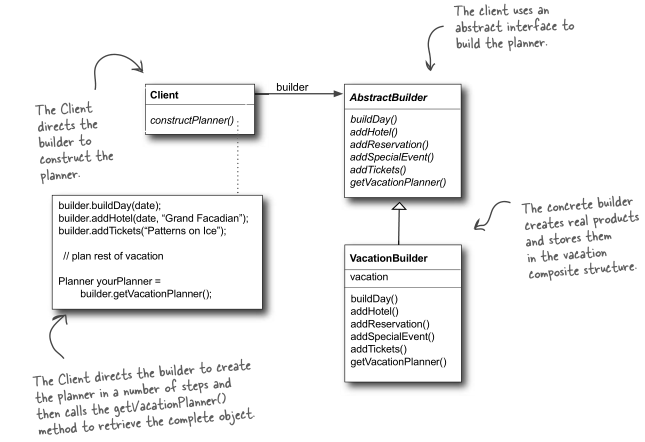
\includegraphics[width=.9\linewidth]{builder/img/builderUML}
	\caption{UML-Darstellung des Builder-Musters}
	\label{fig:builder}
\end{figure}